\chapter{EL GRUPO DE LAS TRANSFORMACIONES}
	\section{Nuevas definiciones y nuevas transformaciones}
		\label{ciclico} 
		Las fórmulas de las transformaciones del apartado \ref{transPsi} quedaron de esta forma:
		\begin{align*}		
		&\text{I}(\sigma(m))\hspace*{-2.4cm}&=& -\sigma(m) + 2\sigma(0)\\
		&\text{T}^\text{k}(\sigma(m))\hspace*{-2.4cm}&=&\ \sigma(m) + \text{k}\\
		&\text{R}(\sigma(m))\hspace*{-2.4cm}&=&\ \sigma(-1-m)
		\end{align*}
			
		Sin embargo, la importancia de estas definiciones radica en qué espectro serial forman, y no en cómo se nombra cada serie específica. No es distinguible a un nivel musical y, de hecho, hay más de un convenio para ello.
		
		Han surgido a lo largo de la historia dos métodos para nombrar las series. El primero, el método tradicional, se ha usado desde al menos 1945. El segundo, el método de tonos absolutos, fue concebido por George Perle en su libro \emph{Twelve Tone Tonality} (1977).
		
		En el método tradicional, T$_0$ se usa para la primera serie que se encuentra en la composición; es decir, la serie original. En cambio, el método de tonos absolutos nombra las series T basándose solamente en la nota en la que comienzan: T$_0$ se usa para la serie que comienza por un Do, y así sucesivamente. En ambas, las series transpuestas se nombran como $\Psi_\text{k}$.
		
		Estas nomenclaturas no caracterizan adecuadamente el objeto matemático que deben representar, es decir, funciones aplicadas a las series. Son nombres arbitrarios que además producen ambigüedad al añadir otras funciones o al intentar describirlo matemáticamente.
		
		En todo caso, cualquier convenio de notación tendrá fórmulas matemáticas distintas al resto, pero todas preservan el material compositivo de la obra. Eso quiere decir que se pueden redefinir algunas de las transformaciones, siempre que preserven el sentido musical. 
		
		Por ejemplo, la inversión puede prescindir de ser transportada para que la primera nota coincida con la original. Para distinguirla de la primera definición, ésta se llamará S de simetría: $\text{S}(\sigma(m)) = -\sigma(m)$.
		
		E igual que la inversión es el cambio de signo por fuera, la retrogradación puede convertirse simplemente en el cambio de signo por dentro. Ésta se llamará V de volteo: $\text{V}(\sigma(m)) = \sigma(-m)$. \footnote{Si no se añade la transformación C, entonces V no conserva el espectro serial de \{I,T,R\}.}
		
		Así quedan dos transformaciones que se asemejan a reflexiones: una por \textit{dentro} y otra por \textit{fuera}; y una adición por \textit{fuera}. Aquí \textit{dentro} significa \textit{antes} de aplicar $\sigma$ y \textit{fuera} significa \textit{después} de aplicar $\sigma$, ya que no se debe olvidar que $\sigma$, la permutación, es una función en sí misma. Y ahora surge una cuestión consecuentemente: ¿cuál sería entonces el resultado de sumar \textit{dentro}, es decir, \textit{antes}?
		
		Esta nueva transformación, cuya aparición resulta natural tras las otras tres, se llama \textit{desplazamiento cíclico}. Inventada y usada por Alban Berg, y en algunas obras primerizas de Schoenberg, C$^\text{k}$ desplaza el comienzo de la serie k posiciones más allá:
		\[\text{C}^\text{k}\left(\sigma\left(m\right)\right)=\sigma\left(m+\text{k}\right)\]		
		\full{$\text{C}^\text{k}=\left(\begin{matrix}0&1&2&&9&10&11\\\sigma\left(\text{k}\right)&\sigma\left(\text{k}+1\right)&\sigma\left(\text{k}+2\right)&\cdots&\sigma\left(\text{k}+9\right)&\sigma\left(\text{k}+10\right)&\sigma\left(\text{k}+11\right)\\\end{matrix}\right)$}
		
		La serie 4-cíclica sobre la permutación P de la Suite Op. 25 es la siguiente serie C$^4$:	
		\[\text{C}^4=\left(\begin{matrix}0&1&2&3&4&5&6&7&8&9&10&11\\6&3&8&2&11&0&9&10&4&5&7&1\\\end{matrix}\right)\]		
		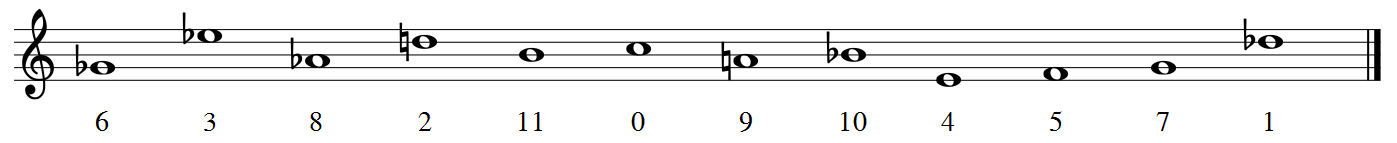
\includegraphics[width=\textwidth]{13.png}
		
		En resumen, se puede trabajar con un nuevo sistema de definiciones que mantienen el significado musical del serialismo pero varían la notación con la que se trabaja. 
		\vspace{-\bigskipamount}
		\begin{multicols}{2}
		\begin{align*}
		\text{S}(\sigma(m)) &= -\sigma(m)\\
		\text{T}^\text{k}(\sigma(m)) &= \sigma(m) + \text{k}
		\end{align*}
		
		\begin{align*}
		\text{V}(\sigma(m)) &= \sigma(-m)\\
		\text{C}^\text{k}(\sigma(m)) &= \sigma(m+\text{k})
		\end{align*}
		\end{multicols}
	
	\section{Diagramas de reloj}
	\label{diagramas}
	
		\begin{wrapfigure}{R}{0.2\textwidth}
			\vspace{-\bigskipamount}
			\begin{tikzpicture}[rotate=30*4,minimum height=0pt,inner sep=0pt,outer sep=0pt,scale=0.65]
			\foreach \x in {0,...,11} {\node at (90-30*\x:2) {\x}; \node (\x) at (90-30*\x:1.6) {};};
			
			\draw [style=flechita] (4)--(5)--(7)--(1)--(6)--(3)--(8)--(2)--(11)--(0)--(9)--(10)--(4);
			
			\node at (0,0) [circle,fill=white] {T$^0$};
			\end{tikzpicture}
			\vspace{-\bigskipamount}
		\end{wrapfigure} Para visualizar mejor cómo actúan las distintas transformaciones, las series se pueden representar mediante \textit{diagramas de reloj}: una sucesión de aristas con una orientación establecida que conecta los vértices de un dodecágono en el orden de la serie. Ya que el desplazamiento cíclico actúa como si la serie fuese circular, hay añadida una arista desde la última nota a la primera. El comienzo de la serie y su orientación se marcan con una flecha.
		
		Arriba se incluye el diagrama de la serie original $\sigma$ de la Suite Op. 25. Se pueden distinguir las características de la serie, como las tres diagonales, que son los tres intervalos de tritono. A continuación se incluyen los diagramas de las transformaciones del apartado \ref{transPsi}: la transposición, la inversión y la retrogradación; así como el nuevo desplazamiento cíclico.
		
		\bigskip
		\hspace*{-0.8cm}
		\begin{tikzpicture}[scale=0.65,rotate=30*4,minimum height=0pt,inner sep=0pt,outer sep=0pt]
		\foreach \x in {0,...,11} {\node at (90-30*\x:2) {\x}; \node (\x) at (90-30*\x:1.6) {};};
		\draw [style=flechita] (5)--(6)--(8)--(2)--(7)--(4)--(9)--(3)--(0)--(1)--(10)--(11)--(5);
		\node at (0,0) [circle,fill=white] {T$^1$};
		
		\foreach \x in {0,...,11} {\node [xshift=3cm] at (90-30*\x:2) {\x}; \node [xshift=3cm] (\x) at (90-30*\x:1.6) {};};
		\draw [style=flechita] (10)--(9)--(0)--(11)--(2)--(8)--(3)--(6)--(1)--(7)--(5)--(4)--(10);
		\node [xshift=3cm] at (0,0) [circle,fill=white] {R};
		
		\foreach \x in {0,...,11} {\node [xshift=6cm] at (90-30*\x:2) {\x}; \node [xshift=6cm] (\x) at (90-30*\x:1.6) {};};
		\draw [style=flechita] (4)--(3)--(1)--(7)--(2)--(5)--(0)--(6)--(9)--(8)--(11)--(10)--(4);
		\node [xshift=6cm] at (0,0) [circle,fill=white] {I};
		
		\foreach \x in {0,...,11} {\node [xshift=9cm] at (90-30*\x:2) {\x}; \node [xshift=9cm] (\x) at (90-30*\x:1.6) {};};		
		\draw [style=flechita] (5)--(7)--(1)--(6)--(3)--(8)--(2)--(11)--(0)--(9)--(10)--(4)--(5);		
		\node [xshift=9cm] at (0,0) [circle,fill=white] {C$^1$};
		\end{tikzpicture}
		\smallskip
		
		La transposición es una rotación en el sentido en el que apunta la flecha; la inversión es una reflexión con el eje de simetría en la diagonal que pasa por la flecha; la retrogradación es un cambio de orientación de la flecha; y el desplazamiento cíclico es el avance interno de la flecha por el recorrido de la serie.		
		
		La diferencia entre las inversiones I y S es precisamente la transposición de $2\sigma(0)=8$ semitonos en este ejemplo. Comparando S con T$^0$ se puede además observar que S es una reflexión con el eje de simetría en 0, en vez de que el eje dependa de la propia permutación.
		
		\begin{center}
			\begin{multicols}{2}
				\begin{tikzpicture}[scale=0.65,rotate=30*4,minimum height=0pt,inner sep=0pt,outer sep=0pt]
				\foreach \x in {0,...,11} {\node at (90-30*\x:2) {\x}; \node (\x) at (90-30*\x:1.6) {};};
				
				\draw [style=flechita] (4)--(3)--(1)--(7)--(2)--(5)--(0)--(6)--(9)--(8)--(11)--(10)--(4);
				
				\node at (0,0) [circle,fill=white] {I};
				\end{tikzpicture}
				
				\begin{tikzpicture}[scale=0.65,rotate=30*4,minimum height=0pt,inner sep=0pt,outer sep=0pt]
				\foreach \x in {0,...,11} {\node at (90-30*\x:2) {\x}; \node (\x) at (90-30*\x:1.6) {};};
				
				\draw [style=flechita] (8)--(7)--(5)--(11)--(6)--(9)--(4)--(10)--(1)--(0)--(3)--(2)--(8);
				
				\node at (0,0) [circle,fill=white] {S};
				\end{tikzpicture}
			\end{multicols}
		\end{center}
	
		Por otro lado, la comparación entre las retrogradaciones R y V muestra que, aunque en principio más arbitraria, V es una transformación más natural, ya que deja fija la flecha. La diferencia entre ellas es en realidad un desplazamiento cíclico de -1.
		
		\begin{center}
			\begin{multicols}{2}
				\begin{tikzpicture}[scale=0.65,rotate=30*4,minimum height=0pt,inner sep=0pt,outer sep=0pt]
				\foreach \x in {0,...,11} {\node at (90-30*\x:2) {\x}; \node (\x) at (90-30*\x:1.6) {};};
				
				\draw [style=flechita] (10)--(9)--(0)--(11)--(2)--(8)--(3)--(6)--(1)--(7)--(5)--(4)--(10);
				
				\node at (0,0) [circle,fill=white] {R};
				\end{tikzpicture}
				
				\begin{tikzpicture}[scale=0.65,rotate=30*4,minimum height=0pt,inner sep=0pt,outer sep=0pt]
				\foreach \x in {0,...,11} {\node at (90-30*\x:2) {\x}; \node (\x) at (90-30*\x:1.6) {};};
				
				\draw [style=flechita] (4)--(10)--(9)--(0)--(11)--(2)--(8)--(3)--(6)--(1)--(7)--(5)--(4);
				
				\node at (0,0) [circle,fill=white] {V};
				\end{tikzpicture}
			\end{multicols}
		\end{center}	
	
	\begin{wrapfigure}{l}{0.2\textwidth}
		\vspace*{-\bigskipamount}
		\qrcode{https://diagramas.netlify.com/}
		%\vspace*{-3\bigskipamount}
	\end{wrapfigure} 

		He creado una página interactiva que genera diagramas de reloj de cualquier serie para cualquier longitud serial, además de generar series aleatorias. También se pueden aplicar las transformaciones a la serie, tanto las originales como las del nuevo sistema, para ver cómo se comporta el diagrama. Está escrita en Elm y el código puede encontrarse en \textit{https://gitlab.com/dodecafonismo/diagramas}.
	
		En el código QR está el enlace de la aplicación web. Sus instrucciones de uso se encuentran al final de la página. El enlace es \textit{https://diagramas.netlify.com/}.
	\bigbreak
	
	\section[El grupo: D$_{12}$ x D$_{12}$]{El grupo: D$_{\textbf{12}}$ x D$_{\textbf{12}}$}
		\label{grupoD}
		El conjunto de transformaciones \{S, T, V, C\} está compuesto por dos parejas con semejanzas entre sí. S es una reflexión y T una rotación de orden 12 -- es decir, que al aplicarla 12 veces se vuelve a la identidad -- y ambas se aplican a la figura entera; es como mover el diagrama por el papel. En cambio, V es una reflexión de la flecha en sí, y C una rotación -- también de orden 12 -- de la flecha sobre la línea; ambas aplicadas al interior de la figura.
		
		Cada pareja genera un grupo muy conocido: el grupo diédrico o diedral. Se denota\footnote{En otros ámbitos, D$_n$ también se denota por D$_{2n}$, ya que $2*n$ es el número de elementos que tiene el grupo.} por D$_{12}$ y representa el grupo de simetrías de un polígono regular; en este caso, un dodecágono. Por ejemplo, aquí se muestran todas las simetrías de un octógono, que son los 16 elementos de D$_{8}$, aplicados a una señal de STOP.
		
		{\tiny\begin{tikzpicture}[scale=1.3]
		\foreach \i in {0,...,7}
		\node[regular polygon,regular polygon sides=8,draw,rotate=-45*\i] at (\i,1) {STOP};
		\foreach \i in {0,...,7}
		\node[regular polygon,regular polygon sides=8,draw,rotate=-45*\i,xscale=-1] at (\i,0) {STOP};		
		\end{tikzpicture}}
	
		De igual manera, el conjunto de series de un espectro serial se consigue aplicando a la serie las distintas funciones transformativas; se obtiene entonces un grupo diédrico para ambas parejas de funciones. 
		
		Al haber dos parejas distintas que actúan por separado dentro y fuera de la figura, el grupo completo que forman las cuatro transformaciones es el producto directo de dos copias del diédrico: D$_{12}\times\text{D}_{12}$.
		
		Podemos observarlo claramente si representamos la serie de una segunda forma: como la correspondencia entre vértices de dos dodecágonos. La serie original, que es en realidad una permutación de 12 elementos, se representa como una función: los vértices del dodecágono interno se envían biyectivamente a los vértices externos. Así, $m \longmapsto \sigma(m)$. Este diagrama es similar al matricial pero enroscado en sí mismo, de tal forma que se aprecia la permutación escogida mediante las flechas, que son fijas, y facilita un significado del antes y el después de aplicarla.
		
		Las dos primeras figuras describen esto mismo: la representación de la serie original y la representación de la permutación mediante las flechas, que se mantendrán constantes en el resto de figuras.
		
			
		{\small \begin{multicols}{2}
			\begin{tikzpicture}[minimum height=18pt,inner sep=0,scale=0.85]
			\draw foreach \x in {0,...,11} {(90-30*\x:2.5) node[very thin,circle,draw] (\x) {\x}};
			\draw foreach \x in {0,...,11} {(90-30*\x:1.25) node[very thin,circle,draw] {\x}};
			\foreach \y/\x in {0/4,1/5,2/7,3/1,4/6,5/3,6/8,7/2,8/11,9/0,10/9,11/10} {\draw [style=flache] (90-30*\y:1.25) -- (\x);};		
			
			\node at (0,0) [very thin,draw,circle,fill=white] {T$^0$};
			\end{tikzpicture}
			
			\begin{tikzpicture}[minimum height=18pt,inner sep=0,scale=0.85]
			\draw foreach \x in {0,...,11} {(90-30*\x:2.5) node (\x) {}};
			\foreach \y/\x in {0/4,1/5,2/7,3/1,4/6,5/3,6/8,7/2,8/11,9/0,10/9,11/10} {\draw [style=flache] (90-30*\y:1.25) -- (\x);};
			\end{tikzpicture}
		\end{multicols}}
	
		Las cuatro siguientes figuras representan las cuatro funciones transformativas, que son en realidad la reflexión y la rotación del grupo diédrico de cada dodecágono. Aplicarlo al de dentro es aplicarlo antes de las flechas; antes de la permutación. Aplicarlo fuera es transformar después de las flechas; después de la permutación.
		
		\newpage
	
		{\small \begin{multicols}{2}
			\begin{tikzpicture}[minimum height=18pt,inner sep=0,scale=0.85]
			\draw foreach \x in {0,...,11} {(90-30*\x:2.5) node[circle] (\x) {}};
			\foreach \y/\x in {0/4,1/5,2/7,3/1,4/6,5/3,6/8,7/2,8/11,9/0,10/9,11/10} {\draw [style=flache] (90-30*\y:1.25) -- (\x);};
			
			\draw foreach \x in {0,...,11} {(90+30*\x:2.5) node[very thin,circle,draw] {\x}};
			\draw foreach \x in {0,...,11} {(90-30*\x:1.25) node[very thin,circle,draw] {\x}};
			
			\draw [red,very thick,dash pattern={on 1pt off 4pt on 10pt off 3pt}] (0,-3.5) -- (0,3.5);
			
			\node at (0,0) [very thin,draw,circle,fill=white] {S};
			\end{tikzpicture}
			
			\begin{tikzpicture}[minimum height=18pt,inner sep=0,scale=0.85]
			\draw foreach \x in {0,...,11} {(90-30*\x:2.5) node[circle] (\x) {}};
			\foreach \y/\x in {0/4,1/5,2/7,3/1,4/6,5/3,6/8,7/2,8/11,9/0,10/9,11/10} {\draw [style=flache] (90-30*\y:1.25) -- (\x);};
			
			\draw foreach \x in {0,...,11} {(120-30*\x:2.5) node[very thin,circle,draw] {\x}};
			\draw foreach \x in {0,...,11} {(90-30*\x:1.25) node[very thin,circle,draw] {\x}};
			
			\draw [style=flocho,thick,red,dashed] (90:3) to [bend right=45] (180:3);
			\node at (0,3.25) {};
			
			\node at (0,0) [very thin,draw,circle,fill=white] {T$^1$};
			\end{tikzpicture}
		\end{multicols}
		
		\begin{multicols}{2}
			\begin{tikzpicture}[minimum height=18pt,inner sep=0,scale=0.85]
			\draw foreach \x in {0,...,11} {(90-30*\x:2.5) node (\x) [circle] {}};
			\foreach \y/\x in {0/4,1/5,2/7,3/1,4/6,5/3,6/8,7/2,8/11,9/0,10/9,11/10} {\draw [style=flache] (90-30*\y:1.25) -- (\x);};
			
			\draw foreach \x in {0,...,11} {(90-30*\x:2.5) node[very thin,circle,draw] {\x}};
			\draw foreach \x in {0,...,11} {(90+30*\x:1.25) node[very thin,circle,draw] {\x}};
			
			\draw [red,very thick,dash pattern={on 1pt off 3pt on 7pt off 2pt}] (0,-2) -- (0,2);
			
			\node at (0,0) [very thin,draw,circle,fill=white] {V};
			\end{tikzpicture}
			
			\begin{tikzpicture}[minimum height=18pt,inner sep=0,scale=0.85]
			\draw foreach \x in {0,...,11} {(90-30*\x:2.5) node[circle] (\x) {}};
			\foreach \y/\x in {0/4,1/5,2/7,3/1,4/6,5/3,6/8,7/2,8/11,9/0,10/9,11/10} {\draw [style=flache] (90-30*\y:1.25) -- (\x);};
			
			\draw foreach \x in {0,...,11} {(90-30*\x:2.5) node[very thin,circle,draw] {\x}};
			\draw foreach \x in {0,...,11} {(60-30*\x:1.25) node[very thin,circle,draw] {\x}};
			
			\draw [style=flocho,thick,red,dashed] (90:1.75) to [bend left=45] (0:1.75);
			
			\node at (0,0) [very thin,draw,circle,fill=white] {C$^1$};
			\end{tikzpicture}
		\end{multicols}
	}
	\newpage
	\section{Conmutatividad entre los elementos del grupo}
	\label{conmut}
		% comprobar cosos que conmutan, mencionar cosos que conmutan en el otro sistema
		
		La rotación (r) y la reflexión (s) de un grupo diédrico no conmutan, sino que cumplen esta relación: $r\cdot s=s\cdot r^{-1}$. Por otro lado, en los productos directos los elementos de un lado conmutan con los del otro. De esta forma, \{S, T\} no conmutan y \{V, C\} tampoco, pero el resto de parejas de transformaciones deben conmutar. Las verificaciones de estas afirmaciones, que confirman que el grupo formado es D$_{12}\times\text{D}_{12}$, se encuentran en el Anexo \ref{app:commm}, página \pageref{app:commm}.
		
		Volviendo a las definiciones originales, al conjunto de transformaciones \{I, T, R, C\}, su estructura interna es bien distinta. El problema de I, a un nivel matemático, es que depende de la permutación escogida, por lo que a veces tiene unas propiedades y a veces otras. En cambio, la definición de V con respecto a R es meramente estética. Ya que no depende de la permutación, su conmutatividad se mantiene invariante. 
		
		Viendo cómo conmutan los elementos de este sistema se aprecia la dificultad definitoria de I. Curiosamente, la conmutatividad de \{I, R\} e \{I, C\} se pierden, pero se gana la de \{I, T\}. Así, T conmuta con todo en el sistema. Esto refleja que en realidad la motivación de la definición de I viene por esta conmutatividad.
		
		 \underline{I y R ya no conmutan:}
		 \vspace{-2\bigskipamount}
		\begin{multicols}{2}
			\begin{align*}
		&\ \text{I}\circ\text{R}(\sigma(m))\\
		=&\ \text{I}(\text{R}(\sigma(m)))\\
		=&\ -\text{R}(\sigma(m))+2\text{R}(\sigma(0))\\
		=&\ -\sigma(-1-m)+2\sigma(-1-0)\\
		=&\ -\sigma(-1-m)+2\sigma(-1)
		\end{align*}
		
		\begin{align*}
		&\ \text{R}\circ\text{I}(\sigma(m))\\
		=&\ \text{R}(\text{I}(\sigma(m)))\\
		=&\ \text{R}(-\sigma(m)+2\sigma(0))\\
		\overset{\footnotemark}{=}&\ \text{R}(-\sigma(m))+2\sigma(0)\\
		=&\ -\sigma(-1-m)+2\sigma(0)
		\end{align*}
		\end{multicols}
		\footnotetext{R y T conmutan.}
		
		Los únicos casos en los que podrían conmutar ocurrirían cuando
		\begin{align*}
		2\sigma\left(0\right)\equiv2\sigma(-1)\ \text{(mod. 12)}&\impliedby\\
		12+2\sigma\left(0\right)=2\sigma\left(-1\right)&\Longleftrightarrow\\
		6+\sigma\left(0\right)=\sigma\left(-1\right)&\Longleftrightarrow\\
		\sigma\left(-1\right)-\sigma\left(0\right)=6&
		\end{align*}
		
		Es decir, cuando la primera y la última nota de la serie original se distancian en 6 semitonos, como es el caso de la permutación en la Suite Op. 25:
		
		\[
		\text{IR}=\text{RI}=\left(\begin{matrix}0&1&2&3&4&5&6&7&8&9&10&11\\10&11&8&9&6&0&5&2&7&1&3&4\\\end{matrix}\right)
		\]	
		
		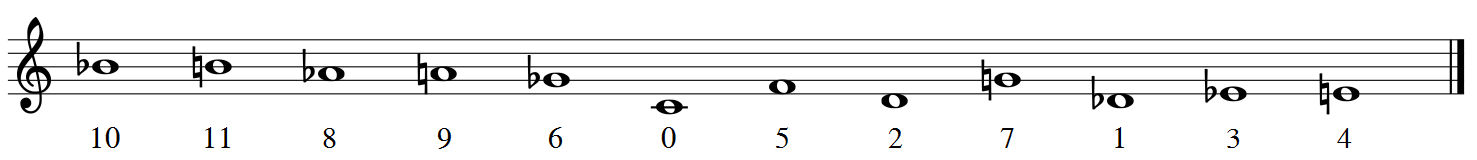
\includegraphics[width=\textwidth]{5.png}\\
		
		 \underline{I y C ya no conmutan:}
		\vspace{-2\bigskipamount}
		\begin{multicols}{2}
			\begin{align*}
			&\ \text{I}\circ\text{C}(\sigma(m))\\
			=&\ \text{I}(\sigma(m+1))\\
			=&\ -\sigma(m+1)+2\sigma(1)
			\end{align*}
			
			\begin{align*}
			&\ \text{C}\circ\text{I}(\sigma(m))\\
			=&\ \text{C}(-\sigma(m)+2\sigma(0))\\
			\overset{\footnotemark}{=}&\ \text{C}(-\sigma(m))+2\sigma(0)\\
			=&\ -\sigma(m+1)+2\sigma(0)
			\end{align*}
		\end{multicols}
		\footnotetext{C y T conmutan.}
		
		Los únicos casos en los que podrían conmutar son cuando
		\begin{align*}
		2\sigma\left(0\right)\equiv2\sigma(1)\ \text{(mod. 12)}&\impliedby\\
		12+2\sigma\left(0\right)=2\sigma\left(1\right)&\Longleftrightarrow\\
		6+\sigma\left(0\right)=\sigma\left(1\right)&\Longleftrightarrow\\
		\sigma\left(1\right)-\sigma\left(0\right)=6&
		\end{align*}
		
		Es decir, cuando la primera y la segunda nota de la serie original se distancian en 6 semitonos.
		
		Si se echan las cuentas con C$^\text{k}$ en vez de con C$^1$, pueden conmutar si $\sigma\left(\text{k}\right)-\sigma\left(0\right)=6$. Como $\sigma$ es una permutación, devuelve todos los valores de 0 a 11 y solamente una vez cada uno. Por tanto, también devuelve 6 + $\sigma(0)$, así que \textbf{siempre existe un único k para el que I y C$^\text{k}$ conmutan}. En el caso de la permutación de la Suite Op. 25, como $\sigma\left(0\right)=4$ hay que encontrar el k para el que $\sigma\left(\text{k}\right)=4+6=10$. En este caso, $\text{k}=11$, pero depende por completo de la permutación original.\\
		
		 \underline{I y T ahora sí conmutan:}
		 \vspace*{-2\bigskipamount}
		\begin{multicols}{2}
			\begin{align*}
			&\ \text{I}\circ\text{T}(\sigma(m))\\
			=&\ \text{I}(\sigma(m)+1)\\
			=&\ -(\sigma(m)+1) + 2(\sigma(0)+1)\\
			=&\ -\sigma(m)-1+2\sigma(0)+2\\
			=&\ -\sigma(m)+2\sigma(0)+1
			\end{align*}
			
			\begin{align*}
			&\ \text{T}\circ\text{I}(\sigma(m))\\
			=&\ \text{T}(-\sigma(m)+2\sigma(0))\\
			=&\ -\sigma(m)+2\sigma(0)+1
			\end{align*}
		\end{multicols}
		
		 \underline{R y C no conmutan:}
		 \vspace*{-2\bigskipamount}
		\begin{multicols}{2}
		\begin{align*}
		&\ \text{R}\circ\text{C}(\sigma(m))\\
		=&\ \text{R}(\sigma(m+1))\\
		=&\ \sigma(-(m+1)-1)\\
		=&\ \sigma(-m-2)
		\end{align*}
		
		\begin{align*}
		&\ \text{C}\circ\text{R}(\sigma(m))\\
		=&\ \text{C}(\sigma(-m-1))\\
		=&\ \sigma(-m-1+1)\\
		=&\ \sigma(-m)
		\end{align*}
		\end{multicols}
		
		 \underline{T y R conmutan:}
		 \vspace*{-2\bigskipamount}
		\begin{multicols}{2}
			\begin{align*}
			&\ \text{T}\circ\text{R}(\sigma(m))\\
			=&\ \text{T}(\sigma(-m-1))\\
			=&\ \sigma(-m-1)+1
			\end{align*}
			
			\begin{align*}
			&\ \text{R}\circ\text{T}(\sigma(m))\\
			=&\ \text{R}(\sigma(m)+1)\\
			=&\ \sigma(-m-1)+1
			\end{align*}
		\end{multicols}
	
		 \underline{T y C conmutan:}
		 \vspace*{-2\bigskipamount}
		\begin{multicols}{2}
			\begin{align*}
			&\ \text{T}\circ\text{C}(\sigma(m))\\
			=&\ \text{T}(\sigma(m+1))\\
			=&\ \sigma(m+1)+1
			\end{align*}
			
			\begin{align*}
			&\ \text{C}\circ\text{T}(\sigma(m))\\
			=&\ \text{V}(\sigma(m)+1)\\
			=&\ \sigma(m+1)+1
			\end{align*}
		\end{multicols}